\documentclass[10pt,journal,compsoc]{IEEEtran}

\ifCLASSOPTIONcompsoc
  \usepackage[nocompress]{cite}
\else
  \usepackage{cite}
\fi

\usepackage[T1]{fontenc}
\usepackage[utf8]{inputenc}
\usepackage{amsmath,amssymb,amsfonts,amsthm}
\usepackage{mathtools}
\usepackage{graphicx}
\usepackage{booktabs}
\usepackage{multirow}
\usepackage{array}
\usepackage{xcolor}
\usepackage{url}
\usepackage[hidelinks]{hyperref}
\pdfstringdefDisableCommands{%
  \def\QG{QuorumGuard}%
  \def\QBench{QuorumBench-50}%
}

\graphicspath{{figures/}}

\newif\ifgoogleaffil
\googleaffiltrue

\newtheorem{theorem}{Theorem}
\newtheorem{lemma}{Lemma}
\newtheorem{proposition}{Proposition}
\newtheorem{corollary}{Corollary}
\theoremstyle{definition}
\newtheorem{definition}{Definition}
\theoremstyle{remark}
\newtheorem{remark}{Remark}

\newcommand{\QG}{\textsc{QuorumGuard}}
\newcommand{\QBench}{\textsc{QuorumBench-50}}
\newcommand{\Neff}{N_{\mathrm{eff}}}
\newcommand{\Hans}{H_{\mathrm{ans}}}
\newcommand{\Htilde}{\tilde{H}_{\mathrm{ans}}}
\newcommand{\phicrit}{\phi_{\mathrm{crit}}}
\newcommand{\betaherd}{\beta_{\mathrm{herd}}}
\newcommand{\CVaR}{\operatorname{CVaR}}
\newcommand{\Cov}{\operatorname{Cov}}
\newcommand{\Prob}{\mathbb{P}}
\newcommand{\E}{\mathbb{E}}
\newcommand{\R}{\mathbb{R}}
\newcommand{\Ind}{\mathbb{I}}

\newcommand{\QBFastSOne}{\ensuremath{46.0\%}}
\newcommand{\QBFastSTwo}{\ensuremath{56.0\%}}
\newcommand{\QBFastJoint}{\ensuremath{28.0\%}}
\newcommand{\QBFastTrap}{\ensuremath{6.7\%}}
\newcommand{\QBFastMean}{\ensuremath{1.11\text{s}}}
\newcommand{\QBFastPNinetyFive}{\ensuremath{1.46\text{s}}}
\newcommand{\QBFastCVaR}{\ensuremath{1.49\text{s}}}

\newcommand{\QBCVaRSOne}{\ensuremath{46.0\%}}
\newcommand{\QBCVaRSTwo}{\ensuremath{52.0\%}}
\newcommand{\QBCVaRJoint}{\ensuremath{28.0\%}}
\newcommand{\QBCVaRTrap}{\ensuremath{6.7\%}}
\newcommand{\QBCVaRMean}{\ensuremath{5.60\text{s}}}
\newcommand{\QBCVaRPNinetyFive}{\ensuremath{5.60\text{s}}}
\newcommand{\QBCVaRCVaR}{\ensuremath{5.60\text{s}}}

\newcommand{\QBSyncSOne}{\ensuremath{66.0\%}}
\newcommand{\QBSyncSTwo}{\ensuremath{68.0\%}}
\newcommand{\QBSyncJoint}{\ensuremath{42.0\%}}
\newcommand{\QBSyncTrap}{\ensuremath{23.3\%}}
\newcommand{\QBSyncMean}{\ensuremath{36.34\text{s}}}
\newcommand{\QBSyncPNinetyFive}{\ensuremath{49.86\text{s}}}
\newcommand{\QBSyncCVaR}{\ensuremath{51.40\text{s}}}

\newcommand{\QBHPRSOne}{\ensuremath{84.0\%}}
\newcommand{\QBHPRSTwo}{\ensuremath{88.0\%}}
\newcommand{\QBHPRJoint}{\ensuremath{72.0\%}}
\newcommand{\QBHPRTrap}{\ensuremath{63.3\%}}
\newcommand{\QBHPRMean}{\ensuremath{35.97\text{s}}}
\newcommand{\QBHPRPNinetyFive}{\ensuremath{48.86\text{s}}}
\newcommand{\QBHPRCVaR}{\ensuremath{51.20\text{s}}}

\newcommand{\QBQGSOne}{\ensuremath{84.0\%}}
\newcommand{\QBQGSTwo}{\ensuremath{88.0\%}}
\newcommand{\QBQGJoint}{\ensuremath{72.0\%}}
\newcommand{\QBQGTrap}{\ensuremath{63.3\%}}
\newcommand{\QBQGMean}{\ensuremath{10.10\text{s}}}
\newcommand{\QBQGPNinetyFive}{\ensuremath{14.82\text{s}}}
\newcommand{\QBQGCVaR}{\ensuremath{16.11\text{s}}}
\newcommand{\QBQGSpeedup}{\ensuremath{3.36\times}}

\hyphenation{Quorum-Guard Paged-Attention multi-agent strag-gler geneal-ogy asyn-chro-nous}

\begin{document}

\title{QuorumGuard: Straggler-Induced Herding Bounds and Claim-Genealogy-Gated Hedged Quorums in Asynchronous Multi-Agent LLM Consensus}

\author{Mohammed~Kamran~Syed%
\IEEEcompsocitemizethanks{\IEEEcompsocthanksitem
\ifgoogleaffil
M.~K.~Syed is with Google, Mountain View, CA, USA (e-mail: syed.kamran@live.com).
\else
M.~K.~Syed is an Independent Systems Researcher (e-mail: syed.kamran@live.com).
\fi\protect\\
Code and scheduler package: \url{https://github.com/batistado/quorumguard} and \url{https://huggingface.co/batistado/QuorumGuard}; \textup{\textsc{QuorumBench}} dataset: \url{https://huggingface.co/datasets/batistado/QuorumBench}; interactive explorer: \url{https://huggingface.co/spaces/batistado/QuorumGuard-Explorer}.}}

\markboth{SUBMITTED FOR ARCHIVAL PUBLICATION, NOVEMBER 2026}%
{SYED: QUORUMGUARD: STRAGGLER-INDUCED HERDING BOUNDS AND CLAIM-GENEALOGY-GATED HEDGED QUORUMS}

\IEEEtitleabstractindextext{%
\begin{abstract}
Multi-agent Large Language Model (LLM) workflows run parallel committees of reasoning and tool-using agents across multi-stage directed acyclic graphs (DAGs) for code verification, numerical auditing, and incident diagnosis. Waiting for synchronous $N$-of-$N$ barriers inflates $\mathrm{P95}$ and $\mathrm{P99}$ latency because container startups, sandboxed tool calls, and long Chain-of-Thought (CoT) traces produce heavy-tailed completion times. Borrowing from replicated storage, serving orchestrators apply asynchronous $k$-of-$N$ fast quorums that commit as soon as the earliest $k$ agents agree and cancel remaining stragglers. In multi-agent LLM pools, however, replica completion time $T_i$ and response accuracy $1 - \varepsilon_i$ have positive covariance ($\Cov(T_i, 1 - \varepsilon_i) > 0$): zero-CoT guesses and shared context echoes return first, while multi-step derivations and code-execution checks arrive in the tail. We prove (Theorem~1) that even when the full population is majority-reliable ($\bar{p} < 0.5$, so synchronous $N$-of-$N$ error decays exponentially to $0$), static $k$-of-$N$ fast quorums undergo an order-statistic phase transition below a critical ratio $\phicrit$, converging to false consensus with probability $1$ as $N \to \infty$ and amplifying downstream herding errors across $M$-stage DAGs (Theorem~2).

We present \QG{}, an event-driven consensus controller and GPU priority-preemption scheduler built on three mechanisms: (1)~pre-commitment semantic entropy gating, which evaluates option-space Shannon entropy $\Hans$ and top-2 logit margins $\Delta$ before any answer letter is generated, avoiding a $70\times$ post-generation self-conditioning collapse; (2)~claim-genealogy quorum sizing ($\Neff$), which tracks upstream provenance DAGs so correlated echoes count as at most one root; and (3)~token-bucket priority dissent boosting, which elevates \texttt{vLLM} decode priority ($\mathrm{Priority}=-10$) for in-flight deep verifiers when early arrivals dissent, share lineage, or fail entropy checks (Theorem~3). Evaluated on Apple M5 Pro Metal GPUs across \texttt{Qwen2.5-3B}, \texttt{Qwen2.5-7B}, and \texttt{Qwen2.5-Coder-14B} with isolated Python sandboxes, \QG{} improves joint two-stage accuracy by $+40.0$--$44.0$ percentage points ($2.50\times$--$2.57\times$, and $63.3\%$ vs.\ $6.7\%$ on boundary traps) over fast $k$-of-$N$ quorums and static $\CVaR$ cutoffs, exceeds unweighted synchronous $N$-of-$N$ voting by $+30.0$ percentage points, matches synchronous genealogy-weighted accuracy ($72.0\%$ on \QBench{}), and reduces $\mathrm{P95}$ and $\CVaR_{0.95}$ workflow latency by $3.19\times$--$3.67\times$, with 8-token GPU quantum preemption compressing straggler queue waits by $4.35\times$--$6.01\times$.
\end{abstract}

\begin{IEEEkeywords}
Multi-agent LLM consensus, asynchronous quorums, tail latency, straggler mitigation, epistemic herding, error cascades, claim genealogy, semantic entropy, GPU priority scheduling.
\end{IEEEkeywords}}

\maketitle
\IEEEdisplaynontitleabstractindextext
\IEEEpeerreviewmaketitle

% ============================================================================
\IEEEraisesectionheading{\section{Introduction}\label{sec:intro}}
% ============================================================================

\IEEEPARstart{M}{ulti-agent} Large Language Model (LLM) systems execute parallel committees of specialized agents across multi-stage workflow Directed Acyclic Graphs (DAGs)~\cite{du2024debate,chen2024reconcile,zheng2024sglang,cemri2025mast}. In code review, numerical validation, and database query auditing, an upstream stage launches $N$ agents combining lightweight triage models, Chain-of-Thought (CoT) reasoners, and sandboxed code verifiers, then passes its committed output to a downstream synthesis or deployment stage~\cite{jain2025livecodebench,luo2025autellix}.

Synchronizing all $N$ agents at a barrier exposes every workflow stage to the slowest straggler $T_{(N)} = \max_{1 \le i \le N} T_i$~\cite{dean2013tail}. Because CoT trace lengths, subprocess sandboxes, and multi-tenant GPU queues are heavy-tailed, full barriers increase $\mathrm{P95}$ latency by $4\times$--$8\times$ over median single-agent execution and spend $40\%$--$60\%$ of GPU tokens on routine steps where lightweight models already agree~\cite{fu2024dynasor,feng2026readiness}. Distributed storage systems such as Fast Paxos~\cite{lamport2006fastpaxos}, Dynamo~\cite{decandia2007dynamo}, Cassandra~\cite{lakshman2010cassandra}, Raft~\cite{ongaro2014raft}, and redundancy-$d$ queues~\cite{gardner2015redundancy,shah2016redundant} avoid this tail penalty through asynchronous $k$-of-$N$ fast quorums that commit once the earliest $k < N$ replicas concur and cancel slower tasks.

\begin{figure*}[!t]
  \centering
  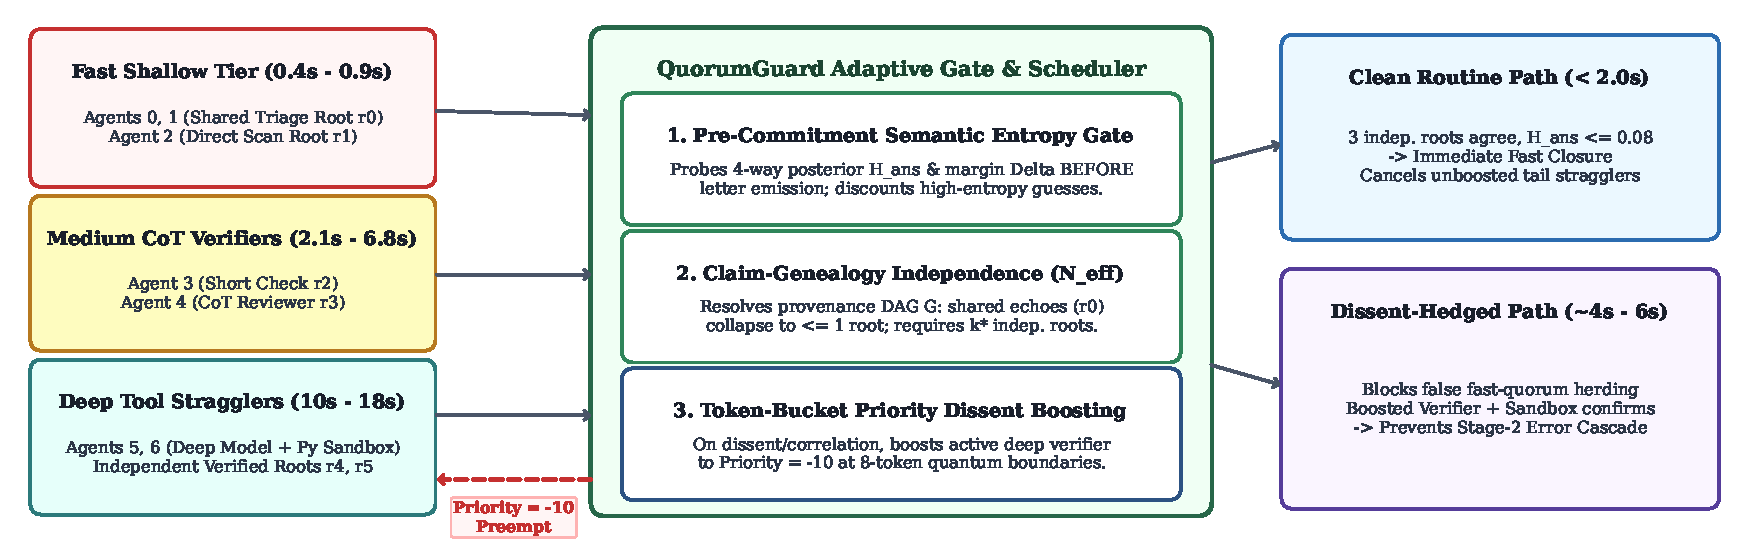
\includegraphics[width=0.98\textwidth]{fig0_architecture.pdf}
  \caption{\QG{} overview. Fast shallow agents ($0.4\text{s}$--$0.9\text{s}$) return early but exhibit shared triage echoes ($r_0$) and boundary-trap errors, while tool-verified \texttt{14B-Coder} agents ($10\text{s}$--$19\text{s}$) arrive in the tail. \QG{} gates early closure using (1)~pre-commitment 4-option posterior entropy $\Hans$ and logit margin $\Delta$, (2)~provenance-DAG effective quorum support $\Neff(t, c; G)$, and (3)~token-bucket \texttt{vLLM} priority preemption ($\mathrm{Priority}=-10$) for active deep stragglers when early arrivals dissent or fail gating.}
  \label{fig:arch}
\end{figure*}

\subsection{Failure of Latency--Correctness Independence}
Classical fast-quorum guarantees assume that replica completion time $T_i$ and response correctness $1 - \varepsilon_i$ are statistically independent ($\Cov(T_i, 1 - \varepsilon_i) = 0$). A storage replica delayed by a network retransmission or garbage-collection pause holds the same data distribution as a fast replica.

In heterogeneous and tool-using LLM pools, completion latency and accuracy covary positively ($\Cov(T_i, 1 - \varepsilon_i) > 0$). Consider task \texttt{T01\_uint16\_overflow} from \QBench{}~\cite{syed2026quorumbench}, which asks for the value stored in \texttt{uint16\_t total\_tokens = batch\_size * seq\_len} in C/CUDA when both inputs equal $256$:
\begin{enumerate}
  \item \emph{Early arrivals ($0.5\text{s}$--$0.9\text{s}$):} Zero-CoT \texttt{Qwen2.5-3B} scanners and triage agents reading a shared static-lint note ($256 \times 256 = 65{,}536$) finish under one second and vote \texttt{65536}.
  \item \emph{Verification stragglers ($6.8\text{s}$--$14.3\text{s}$):} A \texttt{Qwen2.5-7B} CoT reviewer and \texttt{Qwen2.5-Coder-14B} agents executing \texttt{np.uint16(256) * np.uint16(256)} in a Python subprocess take longer because they run multi-step checks, finding modulo-$2^{16}$ wraparound to \texttt{0}.
\end{enumerate}
Under a static $3$-of-$7$ fast quorum, the stage commits \texttt{65536} at $t = 0.68\text{s}$, cancels the running sandbox verifiers, and passes an authoritative consensus record to Stage~2, where downstream agents approve the unpatched kernel.

Prior work addresses either tail scheduling or synchronous error cascades in isolation. Tail-aware agentic schedulers, including readiness--release decoupling for $\CVaR$ latency~\cite{feng2026readiness}, \textsc{Autellix}~\cite{luo2025autellix}, and \textsc{Dynasor}~\cite{fu2024dynasor}, schedule threads or apply deadline cutoffs while assuming early release leaves multi-agent consensus accuracy unchanged. Conversely, studies of multi-agent failure traces (\textsc{MAST}~\cite{cemri2025mast}), claim-genealogy cascades (\emph{From Spark to Fire}~\cite{xie2026sparktofire}), hallucination diffusion (\textsc{HPR-Adaptive}~\cite{hpr2026collective}), and epistemic herding~\cite{herding2026cascades} assume synchronous round barriers where all $N$ agents finish before aggregation, paying full straggler latency on every turn.

\subsection{Contributions}
\QG{} couples online epistemic quorum gating with GPU priority preemption (Fig.~\ref{fig:arch}):
\begin{enumerate}
  \item \emph{Order-statistic phase-transition and DAG cascade bounds (\S\ref{sec:theory}):} Lemma~\ref{lem:finite_n} derives the exact finite-$N$ order-statistic error rate via Beta-function identities, and Theorem~\ref{thm:phase} proves that under $\Cov(T_i, 1 - \varepsilon_i) > 0$, static $k$-of-$N$ fast quorums converge to false consensus with probability $1$ as $N \to \infty$ whenever $k/N < \phicrit$, even when synchronous $N$-of-$N$ error decays to $0$. Theorem~\ref{thm:cascade} derives the $M$-stage herding recurrence and the per-stage error ceiling required for workflow stability.
  \item \emph{Pre-commitment entropy and provenance-DAG gating (\S\ref{sec:design}):} We show that probing option logits after free-form answer generation causes a $70\times$ self-conditioning entropy collapse ($0.003$ vs.\ $0.211$), and introduce single-pass pre-commitment hypothesis probing ($\Hans, \Delta$) combined with clone-invariant provenance-DAG quorum support $\Neff(t, c; G)$ (Proposition~\ref{prop:clone}).
  \item \emph{Token-bucket priority dissent boosting (\S\ref{sec:scheduler}):} When early arrivals share lineage, disagree, or exceed entropy bounds, \QG{} holds the quorum gate and elevates in-flight verifiers to \texttt{vLLM} $\mathrm{Priority} = -10$ under a token-bucket budget, bounding both false-consensus risk and normal-traffic queue delay (Theorem~\ref{thm:optimality}).
  \item \emph{\textup{\QBench{}} and MPS contention evaluation (\S\ref{sec:setup}--\S\ref{sec:eval}):} Across $30$-workflow (\texttt{3B+7B}) and $50$-workflow (\texttt{3B+7B+14B-Coder}) two-stage suites~\cite{syed2026quorumbench} plus 8-token GPU quantum contention experiments on Apple M5 Pro, \QG{} gains $+40.0$--$44.0$ percentage points in joint accuracy over fast quorums and $\CVaR$ cutoffs, beats unweighted synchronous voting by $+30.0$ percentage points, matches synchronous genealogy-weighted accuracy ($66.7\%$ and $72.0\%$), and speeds up $\mathrm{P95}$ latency by $3.30\times$--$3.67\times$.
\end{enumerate}

% ============================================================================
\section{Background and Related Work}\label{sec:related}
% ============================================================================

Table~\ref{tab:novelty} compares \QG{} with classical quorum protocols, LLM workflow schedulers, and synchronous cascade defenses.

\begin{table*}[!t]
\centering
\caption{Comparison of Classical Fast Quorums, Agentic Workflow Schedulers, and Multi-Agent Herding Defenses.}
\label{tab:novelty}
\renewcommand{\arraystretch}{1.12}
\resizebox{\textwidth}{!}{%
\begin{tabular}{@{}lccccc@{}}
\toprule
\textbf{System} & \textbf{Sub-Barrier Exit} & \textbf{Handles $\Cov(T_i, \mathrm{Acc}) > 0$} & \textbf{Pre-Commit Entropy Gate} & \textbf{Genealogy $\Neff$ Deduplication} & \textbf{Dissent Straggler Preemption} \\
\midrule
Fast Paxos / Dynamo / Cassandra~\cite{lamport2006fastpaxos,decandia2007dynamo,lakshman2010cassandra} & Yes & No (Assumes $\Cov = 0$) & No & No & No \\
Redundancy-$d$ Hedged Queues~\cite{dean2013tail,gardner2015redundancy,shah2016redundant} & Yes & No (Identical Replicas) & No & No & No \\
\textsc{Autellix}~\cite{luo2025autellix} \& \textsc{Dynasor}~\cite{fu2024dynasor} & Single-Agent / Thread & No & Token Certaindex & No & Thread-Level LAS \\
Readiness--Release $\CVaR$~\cite{feng2026readiness} & Deadline Release & No (Accuracy-Invariant) & No & No & Static Turn Budget \\
Debate / Self-Consistency~\cite{wang2023selfconsistency,du2024debate,chen2024reconcile} & No ($N$-of-$N$ Sync) & No & Confidence Weighting & No & No \\
Spark-to-Fire~\cite{xie2026sparktofire} \& \textsc{HPR-Adaptive}~\cite{hpr2026collective} & No ($N$-of-$N$ Sync) & No & No & Yes (Sync Barrier) & No \\
Herding \& Runaway Cascades~\cite{herding2026cascades} & No ($N$-of-$N$ Sync) & No & Posterior Inoculation & Partial & No \\
\midrule
\QG{} (Ours) & Adaptive $\tau_{\mathrm{QG}}$ & Yes (Theorems~\ref{thm:phase}--\ref{thm:optimality}) & Pre-Commit $\Hans, \Delta$ & Online DAG $\Neff$ & Token-Bucket \texttt{vLLM} Boost \\
\bottomrule
\end{tabular}%
}
\end{table*}

\emph{Fast Quorums and Redundant Queueing:} Fast Paxos~\cite{lamport2006fastpaxos}, Raft~\cite{ongaro2014raft}, and Dynamo~\cite{decandia2007dynamo} commit on $k < N$ intersecting replicas to hide tail delays, while hedged requests~\cite{dean2013tail} and redundancy-$d$ queues~\cite{gardner2015redundancy,shah2016redundant} take the earliest completion $T_{(1)}$ across identical copies. Shah et al.~\cite{shah2016redundant} proved optimality of early straggler cancellation when job outcomes are identically distributed and independent of service duration. In multi-agent LLM committees, service duration scales with model size, CoT length, and external tool verification, violating this independence assumption.

\emph{LLM Serving and Workflow Schedulers:} Inference engines (\texttt{vLLM}~\cite{kwon2023vllm}, \texttt{SGLang}~\cite{zheng2024sglang}, \texttt{Sarathi-Serve}~\cite{agrawal2024sarathi}) optimize PagedAttention and chunked prefill. Above the engine layer, \textsc{Autellix}~\cite{luo2025autellix} reduces DAG head-of-line blocking via least-attained-service scheduling, \textsc{Dynasor}~\cite{fu2024dynasor} halts single-model reasoning paths via \emph{Certaindex}, and Feng et al.~\cite{feng2026readiness} decouple readiness from turn release under priority budgets to minimize mean--$\CVaR$ latency~\cite{rockafellar2000cvar}. Because these schedulers do not model epistemic correlation between latency and correctness, static deadline release drops late tool-verified refutations on hard queries.

\emph{Multi-Agent Consensus and Cascades:} Self-Consistency~\cite{wang2023selfconsistency}, Debate~\cite{du2024debate,liang2024divergent}, and \textsc{ReConcile}~\cite{chen2024reconcile} aggregate synchronous agent answers, while \textsc{MAST}~\cite{cemri2025mast} cataloged correlated reasoning and verification failures across $1{,}600+$ traces. Recent 2026 defenses model claim-genealogy amplification (\emph{From Spark to Fire}~\cite{xie2026sparktofire}), topological hallucination diffusion (\textsc{HPR-Adaptive}~\cite{hpr2026collective}), and inter-round epistemic herding~\cite{herding2026cascades}, all assuming synchronous $N$-of-$N$ round completion.

% ============================================================================
\section{System Model and Impossibility Bounds}\label{sec:theory}
% ============================================================================

\begin{definition}[Asynchronous Epistemic Quorum Stage]\label{def:stage}
A consensus stage launches $N$ parallel agents $\mathcal{A} = \{1, \dots, N\}$ to identify ground-truth hypothesis $c^\star \in \mathcal{C}$ ($|\mathcal{C}| \ge 2$). Agent $i$ finishes at wall-clock time $T_i > 0$ with CDF $F_i(t)$, emitting candidate $Y_i \in \mathcal{C}$, epistemic signals $\Sigma_i$ (pre-commitment logits $z_i \in \R^{|\mathcal{C}|}$, sequence token entropy, and sandbox verification bit $\xi_i \in \{0, 1\}$), and lineage node $v_i$ in provenance DAG $G = (V, E)$. Let $\varepsilon_i = \Ind[Y_i \neq c^\star]$ be agent $i$'s error indicator, and let $T_{(1)} < \dots < T_{(N)}$ be the order statistics of $\{T_i\}_{i=1}^N$ with concomitant error indicators $\varepsilon_{[1]}, \dots, \varepsilon_{[N]}$~\cite{david2003order}.
\end{definition}

To isolate order-statistic selection bias from lineage correlation, consider $N$ independent agents ($F_i = F$) whose conditional error decreases with reasoning/verification time $t$:
\begin{equation}\label{eq:cond_err}
  g(t) \triangleq \Prob(\varepsilon_i = 1 \mid T_i = t) = p_\infty + (p_0 - p_\infty)e^{-\lambda t},
\end{equation}
where $0 \le p_\infty < 0.5 < p_0 \le 1$ and $\lambda > 0$. Here $p_0$ represents zero-CoT error on subtle traps and $p_\infty$ represents deep-verification residual error. For $T_i \sim \mathrm{Exp}(\mu)$ with density $f(t) = \mu e^{-\mu t}$, the marginal population error rate and latency--accuracy covariance are:
\begin{align}
  \bar{p} &= \E[g(T_i)] = p_\infty + (p_0 - p_\infty)\frac{\mu}{\mu + \lambda}, \label{eq:pbar} \\
  \Cov(T_i, 1 - \varepsilon_i) &= -\Cov(T_i, \varepsilon_i) = (p_0 - p_\infty)\frac{\lambda}{(\mu + \lambda)^2} > 0. \label{eq:cov_exact}
\end{align}

\begin{lemma}[Exact Finite-$N$ Order-Statistic Error Identity]\label{lem:finite_n}
Under~\eqref{eq:cond_err} and $T_i \stackrel{\mathrm{i.i.d.}}{\sim} \mathrm{Exp}(\mu)$, the expected error of the $r$-th fastest agent ($1 \le r \le N$) is:
\begin{equation}\label{eq:exact_r}
  \E[\varepsilon_{[r]}] = p_\infty + (p_0 - p_\infty)\frac{\Gamma(N + 1)\,\Gamma\!\left(N - r + 1 + \frac{\lambda}{\mu}\right)}{\Gamma(N - r + 1)\,\Gamma\!\left(N + 1 + \frac{\lambda}{\mu}\right)}.
\end{equation}
As $N \to \infty$ with $k / N \to \phi \in (0, 1]$, the earliest-$k$ mean member error $\bar{p}_{k,N} = \frac{1}{k}\sum_{r=1}^k \E[\varepsilon_{[r]}]$ converges to:
\begin{equation}\label{eq:p_fast_phi}
  p_{\mathrm{fast}}(\phi) = p_\infty + \frac{p_0 - p_\infty}{\phi}\cdot\frac{\mu}{\mu + \lambda}\!\left(1 - (1 - \phi)^{\frac{\mu + \lambda}{\mu}}\right).
\end{equation}
\end{lemma}

\begin{proof}
The $r$-th order statistic $T_{(r)}$ has density $f_{(r)}(t) = \frac{N!}{(r-1)!(N-r)!}(1 - e^{-\mu t})^{r-1}(e^{-\mu t})^{N-r}\mu e^{-\mu t}$~\cite{david2003order}. Integrating $g(t)f_{(r)}(t)$ via $u = e^{-\mu t} \in (0, 1)$ gives
\[
  \E[\varepsilon_{[r]}] = p_\infty + \frac{(p_0 - p_\infty)\Gamma(N+1)}{\Gamma(r)\Gamma(N-r+1)} B\!\left(r,\, N - r + 1 + \frac{\lambda}{\mu}\right),
\]
which reduces to~\eqref{eq:exact_r} via $B(a, b) = \Gamma(a)\Gamma(b)/\Gamma(a+b)$. As $N \to \infty$ with $k/N \to \phi$, $T_{(k)} \xrightarrow{\mathrm{a.s.}} F^{-1}(\phi) = -\frac{1}{\mu}\ln(1 - \phi) \triangleq t_\phi$, so $\bar{p}_{k,N} \to \frac{1}{\phi}\int_0^{t_\phi} g(t)\mu e^{-\mu t}\,dt$, yielding~\eqref{eq:p_fast_phi}.
\end{proof}

\begin{theorem}[Phase Transition of Static $k$-of-$N$ Fast Quorums]\label{thm:phase}
Assume $\bar{p} < 1/2$ in~\eqref{eq:pbar} and $p_0 > 1/2$ ($|\mathcal{C}| = 2$). Let $\mathcal{E}_{\mathrm{sync}}(N) = \Prob\big(\sum_{i=1}^N \varepsilon_i > N/2\big)$ and $\mathcal{E}_{\mathrm{fast}}(k, N) = \Prob\big(\sum_{r=1}^k \varepsilon_{[r]} > k/2\big)$. Then:
\begin{enumerate}
  \item $\mathcal{E}_{\mathrm{sync}}(N) \le \exp\big(-2 N (1/2 - \bar{p})^2\big) \to 0$ as $N \to \infty$.
  \item A unique critical ratio $\phicrit \in (0, 1)$ satisfies $p_{\mathrm{fast}}(\phicrit) = 1/2$.
  \item For any fixed $\phi = k/N < \phicrit$, there exists $c(\phi) > 0$ such that
  \begin{equation}\label{eq:thm1_bound}
    \mathcal{E}_{\mathrm{fast}}(\lfloor \phi N \rfloor, N) \ge 1 - 2\exp\!\big(-c(\phi) N\big) \xrightarrow{N \to \infty} 1.
  \end{equation}
\end{enumerate}
\end{theorem}

\begin{proof}
Part~(1) follows from Hoeffding's inequality since $\bar{p} < 1/2$. For Part~(2), $g(t)$ decreases strictly in $t$, so its conditional mean $p_{\mathrm{fast}}(\phi)$ over $[0, F^{-1}(\phi)]$ decreases strictly in $\phi$ from $\lim_{\phi \to 0^+} p_{\mathrm{fast}}(\phi) = p_0 > 1/2$ to $p_{\mathrm{fast}}(1) = \bar{p} < 1/2$, giving a unique root $\phicrit \in (0, 1)$. For Part~(3), fix $\phi < \phicrit$, let $\delta = p_{\mathrm{fast}}(\phi) - 1/2 > 0$, and pick $\eta > 0$ such that the mean of $g(T)$ on $[0, \tau_+]$ with $\tau_+ = F^{-1}(\phi + \eta)$ exceeds $1/2 + \delta/2$. By Hoeffding's bound on the empirical CDF $\hat{F}_N(\tau_+)$, $\Prob(T_{(k)} > \tau_+) \le \exp(-2\eta^2 N)$. Conditioned on $\{T_{(1)}, \dots, T_{(k)}\}$ with $T_{(k)} \le \tau_+$, the indicators $\varepsilon_{[1]}, \dots, \varepsilon_{[k]}$ are independent Bernoullis whose conditional mean $\hat{\mu}_k = \frac{1}{k}\sum_{r=1}^k g(T_{(r)})$ concentrates around $p_{\mathrm{fast}}(\phi)$ with $\Prob(\hat{\mu}_k \le 1/2 + \delta/2) \le \exp(-c_1 N)$. Applying Hoeffding's inequality conditioned on $\{\hat{\mu}_k > 1/2 + \delta/2\}$ bounds $\Prob(\sum_{r=1}^k \varepsilon_{[r]} \le k/2) \le \exp(-\frac{1}{2}\phi\delta^2 N)$, giving~\eqref{eq:thm1_bound} with $c(\phi) = \min(2\eta^2, c_1, \frac{1}{2}\phi\delta^2) > 0$.
\end{proof}

\begin{remark}[Scaling Paradox]
When $\phi < \phicrit$, adding parallel agents concentrates $T_{(1)}, \dots, T_{(k)}$ closer to $t = 0$. In Fig.~\ref{fig:phase_cascade}(a) at $\phi \approx 0.35$, increasing $N$ from $7$ to $63$ raises fast-quorum false consensus from $61.4\%$ to $88.3\%$ while reducing synchronous error from $28.4\%$ to $4.5\%$.
\end{remark}

\begin{theorem}[Multi-Stage DAG Herding Amplification]\label{thm:cascade}
In an $M$-stage sequential DAG, suppose Stage~$m$ errs with probability $e_{\mathrm{stage}} \in (0, 1)$ when Stage~$m-1$ succeeded, and with probability $\betaherd + (1 - \betaherd)e_{\mathrm{stage}}$ ($\betaherd \in [0, 1)$~\cite{herding2026cascades}) when Stage~$m-1$ committed an error. Then Stage-$M$ error $q_M$ satisfies
\begin{equation}\label{eq:thm2_closed}
  q_M = e_{\mathrm{stage}} \cdot \frac{1 - \rho^M}{1 - \rho}, \qquad \rho \triangleq \betaherd(1 - e_{\mathrm{stage}}) < 1,
\end{equation}
and keeping $q_M \le \epsilon_{\max}$ for all $M \ge 1$ requires
\begin{equation}\label{eq:thm2_thresh}
  e_{\mathrm{stage}} \le \frac{\epsilon_{\max}(1 - \betaherd)}{1 - \epsilon_{\max}\betaherd}.
\end{equation}
\end{theorem}

\begin{proof}
Conditioning on Stage~$m-1$ gives $q_m = q_{m-1}[\betaherd + (1 - \betaherd)e_{\mathrm{stage}}] + (1 - q_{m-1})e_{\mathrm{stage}} = e_{\mathrm{stage}} + \rho q_{m-1}$ with $q_1 = e_{\mathrm{stage}}$, which unrolls to geometric sum~\eqref{eq:thm2_closed}. Requiring $\lim_{M\to\infty} q_M = e_{\mathrm{stage}}/(1 - \rho) \le \epsilon_{\max}$ yields~\eqref{eq:thm2_thresh}.
\end{proof}

% ============================================================================
\section{The \QG{} Architecture and Protocol}\label{sec:design}
% ============================================================================

\subsection{Pre-Commitment Semantic Entropy Gate}\label{sec:pillar1}
Measuring option uncertainty in autoregressive agents requires probing logits before an answer token is generated. If a model first emits text such as \texttt{"A) 65536"} and an orchestrator then appends \texttt{"Final Answer (A/B/C/D):"} to inspect option log-probabilities, $\Prob(Y_i \mid \text{prompt}, \text{emitted\_letter})$ collapses to $\approx 1.0$ ($\Hans < 0.003~\mathrm{nats}$) because the model copies its own prior token. On \texttt{Qwen2.5-3B}, post-generation probing understated normalized option entropy by $70\times$ ($0.003$ vs.\ $0.211$).

\QG{} uses pre-commitment hypothesis probing:
\begin{enumerate}
  \item Zero-CoT fast agents evaluate next-token $\mathrm{FP32}$ logits $z_i = (z_{i,c})_{c \in \mathcal{C}}$ directly on the decision prompt ($0$ generated tokens, $70$--$100~\mathrm{ms}$ on M5 Pro MPS).
  \item CoT and sandbox-verifier agents generate reasoning steps without naming an option letter, and \QG{} probes $z_i$ right before option selection.
\end{enumerate}
Letting $p_{i,c} = \exp(z_{i,c}) / \sum_{c' \in \mathcal{C}} \exp(z_{i,c'})$, normalized Shannon entropy $\Htilde(i) \in [0, 1]$, top-2 logit margin $\Delta_i$, and calibrated vote weight $w_i$ are:
\begin{align}
  \Htilde(i) &= -\frac{1}{\ln |\mathcal{C}|}\sum_{c \in \mathcal{C}} p_{i,c}\ln p_{i,c}, \qquad \Delta_i = z_{i,(1)} - z_{i,(2)}, \label{eq:entropy_margin} \\
  w_i &= \psi_i \cdot \frac{0.55\big(1 - \Htilde(i)\big) + 0.45\tanh(\Delta_i / \tau_\Delta)}{1 + \alpha_{\mathrm{seq}}\max\big(0, \bar{H}_{\mathrm{seq}}(i) - h_0\big)}, \label{eq:weight}
\end{align}
where $\bar{H}_{\mathrm{seq}}(i)$ is mean reasoning-token entropy and the grounding multiplier $\psi_i = \psi(\mathrm{tier}_i, \xi_i)$ equals $1.38$ for sandbox-verified execution ($\xi_i = 1$), $1.12$--$1.18$ for multi-step CoT, and $0.76$ for unverified zero-CoT probes.

\subsection{Claim-Genealogy Effective Quorum Support ($\Neff$)}\label{sec:pillar2}
Confidence gating alone fails when multiple fast agents read the same misleading upstream summary with low entropy. \QG{} tracks a provenance DAG $G = (V, E)$ whose source nodes $\mathcal{R}_0 = \{u \in V : \deg^-(u) = 0\}$ represent independent inputs, independent reasoning chains, or isolated sandboxes, and whose edges record context consumption.

Each completed agent $i \in \mathcal{A}(t) = \{j : T_j \le t\}$ maps to its ancestor root set $\mathcal{R}(i) \subseteq \mathcal{R}_0$. The genealogy-deduplicated support for claim $c \in \mathcal{C}$ at time $t$ is:
\begin{equation}\label{eq:neff}
  \Neff(t, c; G) = \sum_{r \in \mathcal{R}_0} \max_{\substack{i \in \mathcal{A}(t) \\ Y_i = c,\, r \in \mathcal{R}(i)}} \frac{w_i}{|\mathcal{R}(i)|},
\end{equation}
with empty maxima equal to $0$ and distinct root count $K_{\mathrm{root}}(t, c; G) = \big|\bigcup_{i \in \mathcal{A}(t): Y_i = c} \mathcal{R}(i)\big|$.

\begin{proposition}[Clone-Invariance and Submodularity]\label{prop:clone}
For any provenance DAG $G$ and claim $c$: (1)~if $M$ agents consume a shared summary node $s$ with $\mathcal{R}(s) = \{r_0\}$ and weights $w^{(1)}, \dots, w^{(M)} \le w_0$, then $\Neff(t, c; G) \le w_0$ and $K_{\mathrm{root}}(t, c; G) = 1$ for all $M \ge 1$; (2)~for fixed $\{w_i\}$, $S \mapsto \Neff(S, c; G)$ is monotone non-decreasing and submodular over $S \subseteq \mathcal{A}$.
\end{proposition}

\begin{proof}
When agents $1, \dots, M$ trace only to $r_0$, $|\mathcal{R}(m)| = 1$ and~\eqref{eq:neff} has one nonzero term $\max_{1 \le m \le M} w^{(m)} \le w_0$ with $K_{\mathrm{root}} = |\{r_0\}| = 1$. Each per-root term $f_r(S) = \max_{i \in S_c: r \in \mathcal{R}(i)} (w_i / |\mathcal{R}(i)|)$ is a pointwise maximum of non-negative modular coordinate functions and is therefore monotone submodular; summing over $r \in \mathcal{R}_0$ preserves both properties.
\end{proof}

\begin{figure}[!t]
\centering
\footnotesize
\renewcommand{\arraystretch}{1.10}
\begin{tabular}{|p{0.94\columnwidth}|}
\hline
\textbf{Algorithm 1:} \QG{} Consensus Gate and Dissent Preemption \\
\hline
\textbf{Input:} Pool $\mathcal{A}$ ($|\mathcal{A}|=N$), DAG $G$, Budget Pool $\mathcal{B}$, $(k_{\min}, \tau_{\mathrm{eff}}, \gamma_H, \Delta_{\min}, m_{\mathrm{gap}})$. \\
\textbf{State:} $S \leftarrow \emptyset$; \texttt{boosted} $\leftarrow \mathrm{False}$. Launch all $i \in \mathcal{A}$ at \texttt{vLLM} $\mathrm{Priority} = 0$. \\
1: \textbf{while} $|S| < N$ \textbf{on completion event} $(i, Y_i, \Sigma_i)$ at time $t$: \\
2: \hspace{1em} $S \leftarrow S \cup \{i\}$; compute $w_i$ via~\eqref{eq:weight}, $\Neff(t, c; G)$ and $K_{\mathrm{root}}(t, c; G)$ via~\eqref{eq:neff}. \\
3: \hspace{1em} $c_1 \leftarrow \arg\max_c \Neff(t, c; G)$;\quad $c_2 \leftarrow \arg\max_{c \neq c_1} \Neff(t, c; G)$. \\
4: \hspace{1em} $S_{c_1} \leftarrow \{j \in S : Y_j = c_1\}$;\quad $\bar{H}_{c_1} \leftarrow \mathrm{mean}_{S_{c_1}} \Htilde$;\quad $\Delta_{c_1}^{\min} \leftarrow \min_{S_{c_1}} \Delta$. \\
5: \hspace{1em} $\mathrm{dissent} \leftarrow \Ind[\Neff(t, c_2; G) \ge 0.35]$;\quad $R_{\mathrm{deep}} \leftarrow$ deep/verified roots in $S_{c_1}$. \\
6: \hspace{1em} $\mathrm{CleanFast} \leftarrow (\neg\mathrm{dissent}) \wedge (K_{\mathrm{root}}(t, c_1) \ge k_{\min}) \wedge (\Neff(t, c_1) \ge \tau_{\mathrm{eff}}) \wedge (\bar{H}_{c_1} \le \gamma_H) \wedge (\Delta_{c_1}^{\min} \ge \Delta_{\min})$. \\
7: \hspace{1em} $\mathrm{VerifiedHedge} \leftarrow (R_{\mathrm{deep}} \ge 2 \vee (R_{\mathrm{deep}} \ge 1 \wedge \neg\mathrm{dissent})) \wedge (K_{\mathrm{root}}(t, c_1) \ge 2) \wedge (\Neff(t, c_1) - \Neff(t, c_2) \ge m_{\mathrm{gap}})$. \\
8: \hspace{0.65em} \textbf{if} $\mathrm{CleanFast} \vee \mathrm{VerifiedHedge}$ \textbf{then} \\
9: \hspace{1.65em} Cancel $\mathcal{A} \setminus S$; $\mathcal{B}.\mathrm{refill}()$; \textbf{return} $(c_1, t)$. \\
10: \hspace{0.5em} \textbf{if} $\neg\texttt{boosted} \wedge |S| \ge k_{\min}$ \textbf{then} \\
11: \hspace{1.65em} \texttt{boosted} $\leftarrow \mathrm{True}$; $J \leftarrow$ active deep verifiers in $\mathcal{A} \setminus S$. \\
12: \hspace{1.65em} Elevate earliest $\mathcal{B}.\mathrm{try\_acquire}(\min(B_{\mathrm{stage}}, |J|))$ agents in $J$ to $\mathrm{Priority} = -10$. \\
13: $\mathcal{B}.\mathrm{refill}()$; \textbf{return} $(\arg\max_c \Neff(T_{(N)}, c; G),\, T_{(N)})$. \\
\hline
\end{tabular}
\caption{\QG{} adaptive consensus stopping and priority-budget dissent preemption.}\label{fig:alg1}
\end{figure}

\subsection{Token-Bucket Priority Dissent Boosting}\label{sec:scheduler}
Algorithm~1 (Fig.~\ref{fig:alg1}) launches all $N$ agents at normal serving priority ($\mathrm{Priority} = 0$). On routine steps where $k_{\min}$ independent roots agree with $\bar{H}_{c_1} \le \gamma_H$ and $\Delta_{c_1}^{\min} \ge \Delta_{\min}$, $\mathrm{CleanFast}$ commits in $0.7\text{s}$--$1.8\text{s}$ and cancels remaining stragglers. If $k_{\min}$ raw agents finish without passing $\mathrm{CleanFast}$ due to shared roots, split votes, or elevated entropy, Lines~10--12 acquire up to $B_{\mathrm{stage}}$ tokens from a \texttt{PriorityBudgetPool} $\mathcal{B}$ (capacity $B_{\max}$, refill rate $r_{\mathrm{refill}}$/stage) and raise in-flight verifiers to \texttt{vLLM} $\mathrm{Priority} = -10$, preempting normal decode queues at 8-token quantum boundaries. Once boosted verifiers satisfy $\mathrm{VerifiedHedge}$ (Line~7), the stage commits immediately without waiting for $T_{(N)}$.

\begin{theorem}[False-Consensus Risk and Queue-Delay Bound]\label{thm:optimality}
Under Algorithm~1: (1)~if independent low-entropy roots err on the same wrong option with probability at most $\eta_{\mathrm{clean}}$ and escalated verified quorums err with probability at most $\eta_{\mathrm{deep}}$, $M$ clones sharing one flawed root $r_0$ ($k_{\min} \ge 2$) never trigger $\mathrm{CleanFast}$, and stage false-consensus risk satisfies $\mathcal{E}_{\mathrm{QG}} \le \max(\eta_{\mathrm{clean}}^{k_{\min}}, \eta_{\mathrm{deep}})$; (2)~in a preemptive-resume M/G/1 quantum server at load $\rho < 1$, token-bucket admission bounds boosted utilization to $\rho_{\mathrm{hi}} = \lambda_{\mathrm{boost}}\bar{S}_{\mathrm{boost}} \le r_{\mathrm{refill}}\lambda_{\mathrm{stage}}\bar{S}_{\mathrm{boost}} < \rho$, reducing boosted queue wait by factor $(1 - \rho)/(1 - \rho_{\mathrm{hi}})$ vs.\ FCFS while bounding normal-traffic mean wait to $W_{\mathrm{norm}} = W_{\mathrm{FCFS}}/(1 - \rho_{\mathrm{hi}})$.
\end{theorem}

\begin{proof}
By Proposition~\ref{prop:clone}, $M$ echoes of $r_0$ have $K_{\mathrm{root}} = 1 < k_{\min}$, blocking Line~6; passing $\mathrm{CleanFast}$ requires $\ge k_{\min}$ disjoint roots erring simultaneously ($\le \eta_{\mathrm{clean}}^{k_{\min}}$), while escalated stages err at rate $\le \eta_{\mathrm{deep}}$. Part~(2) follows from Cobham's two-class preemptive-resume M/G/1 queue conservation law under token-bucket rate $\lambda_{\mathrm{boost}} \le r_{\mathrm{refill}}\lambda_{\mathrm{stage}}$.
\end{proof}

% ============================================================================
\section{Experimental Setup}\label{sec:setup}
% ============================================================================

All experiments ran on an Apple M5 Pro workstation ($48~\mathrm{GB}$ unified memory, $\mathrm{FP16}$ Metal MPS, PyTorch~2.15.0, \texttt{transformers}~5.22.1) with \texttt{torch.mps.synchronize()} barriers around every timing call. We evaluate two multi-stage pools on \QBench{}~\cite{syed2026quorumbench}:
\begin{enumerate}
  \item \emph{2-tier pilot (\textup{\texttt{3B}} + \textup{\texttt{7B}}, $30$ workflows):} Stage~1 ($N_1 = 7$) runs $3$ zero-CoT \texttt{Qwen2.5-3B-Instruct}~\cite{yang2024qwen25} agents ($2$ sharing triage summary root $r_0$, $1$ independent scanner $r_1$), $1$ short-CoT \texttt{3B} checker ($r_2$), $1$ \texttt{Qwen2.5-7B-Instruct} CoT reviewer ($r_3$), and $2$ \texttt{Qwen2.5-7B} Python-sandbox verifiers ($r_4, r_5$). Stage~2 ($N_2 = 5$) runs $3$ fast \texttt{3B} coordinators ($2$ echoing Stage~1's commit, $1$ reading raw context) and $2$ \texttt{7B} deployment auditors.
  \item \emph{3-tier \textup{\QBench{}} scale-up (\textup{\texttt{3B}} + \textup{\texttt{7B}} + \textup{\texttt{14B-Coder}}, $50$ workflows, $100$ stage evaluations):} Replaces Stage-1 sandbox verifiers ($r_4, r_5$) and Stage-2 auditors with 48-layer \texttt{Qwen2.5-Coder-14B-Instruct}~\cite{hui2024qwen25coder} ($\sim 28.5~\mathrm{GB}$ $\mathrm{FP16}$) alongside Pareto($\alpha=2.25$) container/queue delays.
\end{enumerate}
Sandbox verifiers generate self-contained \texttt{python3} scripts (\texttt{numpy}, \texttt{sqlite3}, fixed-width C integers) executed in isolated \texttt{python3 -I} subprocesses ($2.5\text{s}$ timeout); $\xi_i = 1$ is set only when the subprocess exits with code~$0$ and non-empty stdout.

\QBench{} contains $20$ routine workflows and $30$ boundary-trap workflows inspired by \textsc{LiveCodeBench}~\cite{jain2025livecodebench}, \textsc{MATH}~\cite{hendrycks2021math}, and \textsc{MAST}~\cite{cemri2025mast}, covering \texttt{uint16\_t}/\texttt{int32\_t}/\texttt{int8\_t} wraparound, IEEE-754 \texttt{float32} $2^{24}$ ULP rounding and \texttt{NaN} identity, SQL \texttt{NOT IN (..., NULL)} and \texttt{COUNT(col)} NULL handling, C/Python operator precedence (\texttt{1 << 2 + 3}, \texttt{3 \^{} 4 \% 5}, chained comparisons), closure late-binding, Dijkstra negative edges, and lease clock-skew split-brain windows. Stage-2 options are phrased as neutral deployment actions without diagnostic spoilers. We compare \texttt{Fast k-of-N}~\cite{decandia2007dynamo}, \texttt{CVaR Static Cutoff} ($2.8\text{s}$/stage)~\cite{feng2026readiness}, unweighted \texttt{Sync N-of-N}~\cite{wang2023selfconsistency}, \texttt{Genealogy Sync (HPR)}~\cite{xie2026sparktofire,hpr2026collective}, and \QG{} ($k_{\min} = 3, \tau_{\mathrm{eff}} = 2.12, \gamma_H = 0.08, \Delta_{\min} = 3.2$) under \texttt{seed=2026}.

% ============================================================================
\section{Experimental Results}\label{sec:eval}
% ============================================================================

\begin{figure*}[!t]
  \centering
  \begin{minipage}[t]{0.485\textwidth}
    \centering
    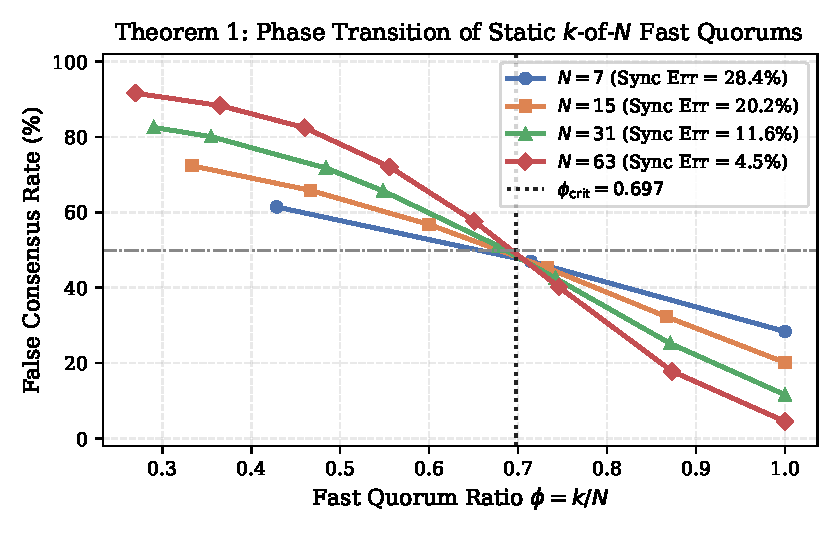
\includegraphics[width=\textwidth]{fig1_phase_transition.pdf}
  \end{minipage}\hfill
  \begin{minipage}[t]{0.485\textwidth}
    \centering
    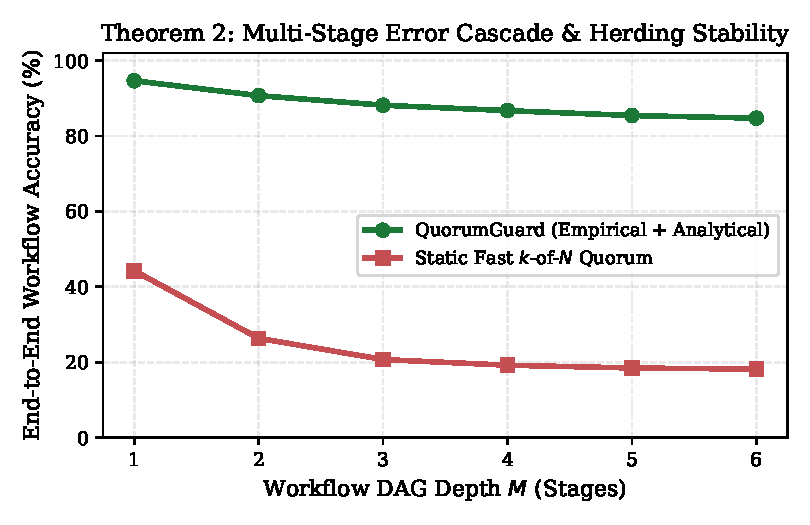
\includegraphics[width=\textwidth]{fig2_cascade_amplification.pdf}
  \end{minipage}
  \caption{Analytical and $40{,}000$-trial Monte Carlo verification of Theorems~\ref{thm:phase} and~\ref{thm:cascade}. (Left) With population mean error $\bar{p} = 0.395 < 0.5$, static $k$-of-$N$ fast quorums cross a phase transition at $\phicrit = 0.697$: below $\phicrit$, scaling $N$ from $7$ to $63$ increases false consensus from $61.4\%$ to $88.3\%$ while synchronous error drops from $28.4\%$ to $4.5\%$. (Right) Across $M = 1 \dots 6$ DAG stages ($\betaherd = 0.72$), fast-quorum accuracy falls to $19.2\%$ by Stage~4 versus $86.7\%$ under \QG{}.}
  \label{fig:phase_cascade}
\end{figure*}

\subsection{Verification of Phase-Transition and Cascade Bounds}
Fig.~\ref{fig:phase_cascade} compares Lemma~\ref{lem:finite_n} and Theorems~\ref{thm:phase}--\ref{thm:cascade} against $40{,}000$ Monte Carlo trials ($p_0 = 0.78, p_\infty = 0.08, \lambda = 0.55, \mu = 0.45$, giving $\bar{p} = 0.3950 < 0.5$, $\Cov(T_i, 1 - \varepsilon_i) = +0.3850$, and $\phicrit = 0.6973$). At $\phi \approx 0.35 < \phicrit$, scaling $N$ from $7$ to $63$ raises static fast-quorum false consensus from $61.4\%$ to $88.3\%$ while synchronous majority error drops from $28.4\%$ to $4.5\%$; analytical member error matches simulation within $3.5 \times 10^{-3}$ at $N = 63$. Across $M \le 6$ DAG stages, Eq.~\eqref{eq:thm2_closed} matches simulated cascade rates within $0.2\%$.

\begin{figure*}[!t]
  \centering
  \begin{minipage}[t]{0.485\textwidth}
    \centering
    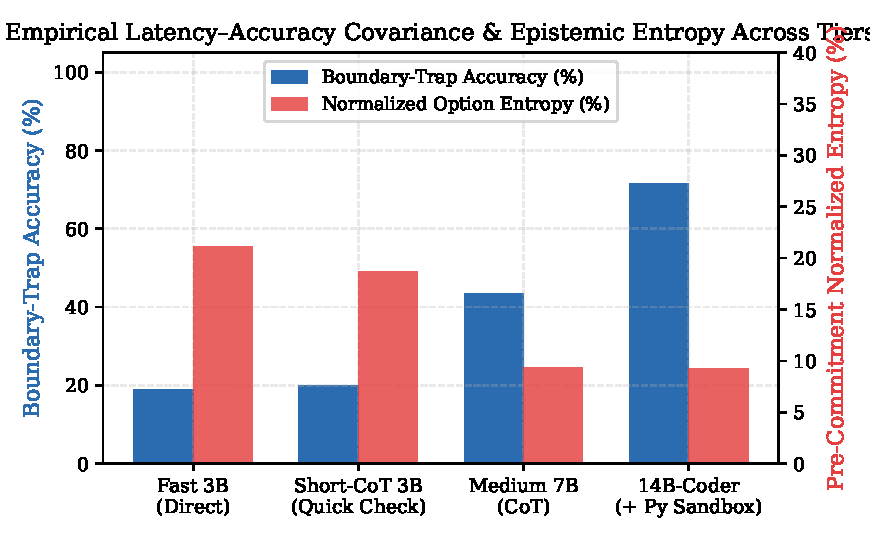
\includegraphics[width=\textwidth]{fig4_entropy_covariance_calibration.pdf}
  \end{minipage}\hfill
  \begin{minipage}[t]{0.485\textwidth}
    \centering
    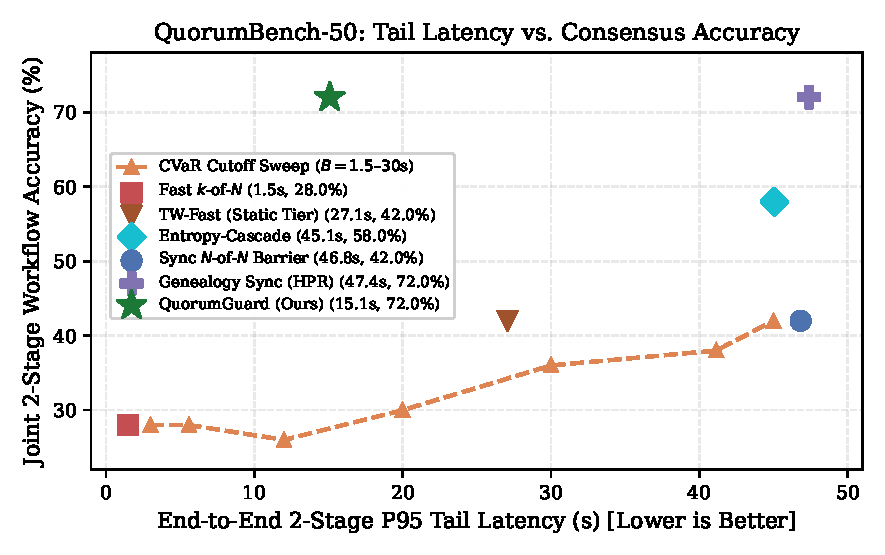
\includegraphics[width=\textwidth]{fig3_pareto_latency_accuracy.pdf}
  \end{minipage}
  \caption{Live Apple M5 Pro MPS telemetry on \QBench{}. (Left) Boundary-trap accuracy and pre-commitment normalized option entropy across the four agent tiers. (Right) Joint two-stage workflow accuracy versus $\mathrm{P95}$ tail latency across all five consensus policies.}
  \label{fig:mps_main}
\end{figure*}

\subsection{Empirical Covariance and Pre-Commitment Entropy}
Live Qwen2.5 executions confirm positive latency--accuracy covariance on both pools. On the 30-task 2-tier suite, $\Cov(T_i, 1 - \varepsilon_i) = +0.7185~\mathrm{s}$ ($r = +0.241$) overall and $+1.4339~\mathrm{s}$ ($r = +0.520$) on boundary traps. On the 50-task 3-tier \QBench{} suite ($350$ Stage-1 runs), $\Cov(T_i, 1 - \varepsilon_i) = +0.9661~\mathrm{s}$ ($r = +0.234$) overall and $+1.5853~\mathrm{s}$ ($r = +0.404$) on boundary traps, while hardware-only MPS inference duration (excluding queue and sandbox overheads) yields $\Cov(T_{\mathrm{MPS}, i}, 1 - \varepsilon_i) = +0.6142~\mathrm{s}$ ($r = +0.206$). Across tiers in Fig.~\ref{fig:mps_main}(Left), \texttt{3B Direct} averages $0.55\text{s}$ ($0.10\text{s}$ MPS, $18.9\%$ trap accuracy, $\Htilde = 0.211$), \texttt{3B Short-CoT} averages $2.69\text{s}$ ($20.0\%$ trap accuracy, $\Htilde = 0.187$), \texttt{7B CoT} averages $6.97\text{s}$ ($43.3\%$ trap accuracy, $\Htilde = 0.094$), and \texttt{14B-Coder + Sandbox} averages $18.91\text{s}$ ($12.93\text{s}$ MPS, $80.0\%$ overall and $71.7\%$ trap accuracy, $\Htilde = 0.093$).

\begin{table*}[!t]
\centering
\caption{Live 30-Workflow Two-Stage MPS Evaluation (\texttt{Qwen2.5-3B} + \texttt{Qwen2.5-7B} + Python Sandbox, $\mathrm{Seed}=2026$).}
\label{tab:pilot30}
\renewcommand{\arraystretch}{1.12}
\resizebox{0.93\textwidth}{!}{%
\begin{tabular}{@{}lccccccc@{}}
\toprule
\textbf{Consensus Policy} & \textbf{Stage-1 Acc} & \textbf{Stage-2 Acc} & \textbf{Joint 2-Stage Acc} & \textbf{Mean Latency} & \textbf{Routine Mean} & \textbf{P95 Latency} & \textbf{$\CVaR_{0.95}$ Latency} \\
\midrule
\texttt{Fast k-of-N Quorum} & $43.3\%$ & $43.3\%$ & $26.7\%$ & $1.07\text{s}$ & $1.03\text{s}$ & $1.41\text{s}$ & $1.43\text{s}$ \\
\texttt{CVaR Static Cutoff}~\cite{feng2026readiness} & $43.3\%$ & $40.0\%$ & $26.7\%$ & $5.60\text{s}$ & $5.60\text{s}$ & $5.60\text{s}$ & $5.60\text{s}$ \\
\texttt{Sync N-of-N Barrier}~\cite{wang2023selfconsistency} & $60.0\%$ & $50.0\%$ & $36.7\%$ & $27.79\text{s}$ & $27.18\text{s}$ & $36.00\text{s}$ & $36.99\text{s}$ \\
\texttt{Genealogy Sync (HPR)}~\cite{xie2026sparktofire,hpr2026collective} & $80.0\%$ & $70.0\%$ & $66.7\%$ & $28.30\text{s}$ & $27.18\text{s}$ & $36.73\text{s}$ & $36.99\text{s}$ \\
\midrule
\QG{} (Ours) & $80.0\%$ & $70.0\%$ & $66.7\%$ & $7.87\text{s}$ & $4.62\text{s}$ & $10.00\text{s}$ & $10.59\text{s}$ \\
\bottomrule
\end{tabular}%
}
\end{table*}

\begin{table*}[!t]
\centering
\caption{\QBench{} Scale-Up Across 50 Two-Stage Workflows ($100$ Stage Evaluations; \texttt{Qwen2.5-3B} + \texttt{7B} + \texttt{14B-Coder} + Python Sandbox).}
\label{tab:scale50}
\renewcommand{\arraystretch}{1.12}
\resizebox{0.93\textwidth}{!}{%
\begin{tabular}{@{}lccccccc@{}}
\toprule
\textbf{Consensus Policy} & \textbf{Stage-1 Acc} & \textbf{Stage-2 Acc} & \textbf{Joint 2-Stage Acc} & \textbf{Trap Joint Acc} & \textbf{Mean Latency} & \textbf{P95 Latency} & \textbf{$\CVaR_{0.95}$ Latency} \\
\midrule
\texttt{Fast k-of-N Quorum} & \QBFastSOne & \QBFastSTwo & \QBFastJoint & \QBFastTrap & \QBFastMean & \QBFastPNinetyFive & \QBFastCVaR \\
\texttt{CVaR Static Cutoff}~\cite{feng2026readiness} & \QBCVaRSOne & \QBCVaRSTwo & \QBCVaRJoint & \QBCVaRTrap & \QBCVaRMean & \QBCVaRPNinetyFive & \QBCVaRCVaR \\
\texttt{Sync N-of-N Barrier}~\cite{wang2023selfconsistency} & \QBSyncSOne & \QBSyncSTwo & \QBSyncJoint & \QBSyncTrap & \QBSyncMean & \QBSyncPNinetyFive & \QBSyncCVaR \\
\texttt{Genealogy Sync (HPR)}~\cite{xie2026sparktofire,hpr2026collective} & \QBHPRSOne & \QBHPRSTwo & \QBHPRJoint & \QBHPRTrap & \QBHPRMean & \QBHPRPNinetyFive & \QBHPRCVaR \\
\midrule
\QG{} (Ours) & \QBQGSOne & \QBQGSTwo & \QBQGJoint & \QBQGTrap & \QBQGMean & \QBQGPNinetyFive & \QBQGCVaR \\
\bottomrule
\end{tabular}%
}
\end{table*}

\subsection{Two-Stage Workflow Accuracy and Tail Latency}
Tables~\ref{tab:pilot30} and~\ref{tab:scale50} summarize end-to-end two-stage consensus performance. Under \texttt{Fast k-of-N}, premature Stage-1 closure drops joint two-stage accuracy to $26.7\%$ on the 30-task suite and $28.0\%$ on \QBench{} ($6.7\%$ on the 30 boundary traps, failing $28/30$ workflows); when Stage~1 commits a wrong claim, Stage~2 errs with probability $\Prob(\text{S2 err} \mid \text{S1 err}) = 0.765$ as fast coordinators follow the upstream consensus record. \texttt{CVaR Static Cutoff} ($2.8\text{s}$/stage) clips the $7\text{s}$--$19\text{s}$ verifiers and stays at $28.0\%$ joint accuracy. Unweighted \texttt{Sync N-of-N} waits $36.34\text{s}$ mean ($49.86\text{s}$ $\mathrm{P95}$) yet reaches only $42.0\%$ joint accuracy ($23.3\%$ on boundary traps) because four fast \texttt{3B} votes outnumber three \texttt{7B}/\texttt{14B} verifiers on shared misconceptions.

\QG{} matches \texttt{Genealogy Sync (HPR)} on every accuracy metric: $80.0\%$ Stage-1 and $66.7\%$ joint accuracy on Table~\ref{tab:pilot30}, and $84.0\%$ Stage-1, $88.0\%$ Stage-2, and $72.0\%$ joint accuracy ($63.3\%$ on boundary traps, $9.45\times$ higher than \texttt{Fast k-of-N}) on Table~\ref{tab:scale50}. At the same time, \QG{} lowers $\mathrm{P95}$ workflow latency from $36.73\text{s}$ to $10.00\text{s}$ ($3.67\times$) on the 2-tier pool and from $48.86\text{s}$--$49.86\text{s}$ to $14.82\text{s}$ ($3.30\times$--$3.36\times$) on \QBench{}, with mean latency dropping $3.56\times$ ($35.97\text{s} \to 10.10\text{s}$).

\begin{table}[!t]
\centering
\caption{Stage-1 Component Ablations ($30$-Workflow Live MPS Telemetry).}
\label{tab:ablation}
\renewcommand{\arraystretch}{1.12}
\resizebox{\columnwidth}{!}{%
\begin{tabular}{@{}lcccc@{}}
\toprule
\textbf{Variant} & \textbf{S1 Acc} & \textbf{Trap Acc} & \textbf{Mean} & \textbf{P95 ($\CVaR_{95}$)} \\
\midrule
1. \texttt{Fast k-of-N} & $43.3\%$ & $5.6\%$ & $0.56\text{s}$ & $0.76\text{s}$ ($0.77\text{s}$) \\
2. \texttt{+ Entropy Gate Only} & $76.7\%$ & $66.7\%$ & $9.30\text{s}$ & $17.24\text{s}$ ($19.04\text{s}$) \\
3. \texttt{+ Genealogy $\Neff$ Only} & $60.0\%$ & $38.9\%$ & $7.08\text{s}$ & $17.34\text{s}$ ($19.12\text{s}$) \\
4. \texttt{\QG{} w/o Boost} & $80.0\%$ & $72.2\%$ & $9.31\text{s}$ & $16.20\text{s}$ ($18.20\text{s}$) \\
5. \texttt{\QG{} (Full)} & $80.0\%$ & $72.2\%$ & $3.70\text{s}$ & $5.93\text{s}$ ($6.35\text{s}$) \\
\bottomrule
\end{tabular}%
}
\end{table}

\begin{figure}[!t]
  \centering
  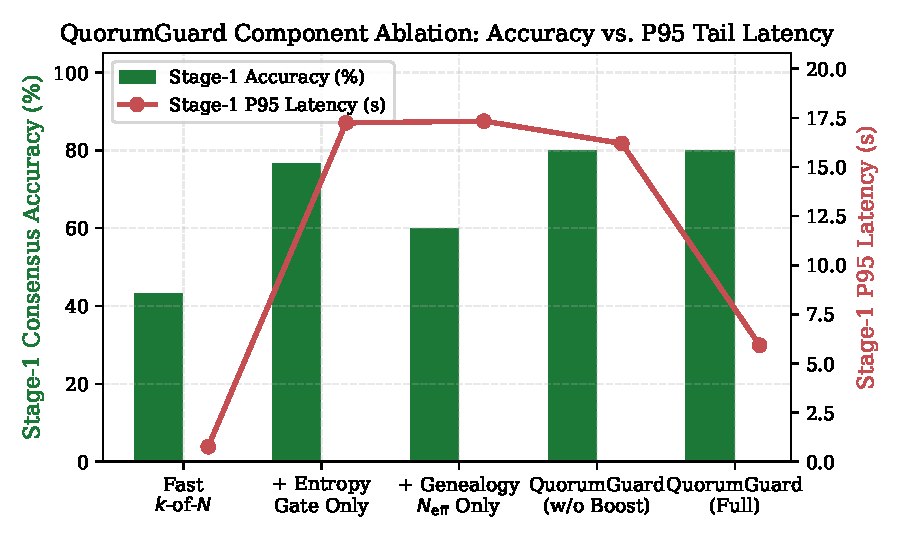
\includegraphics[width=0.96\columnwidth]{fig5_ablation_breakdown.pdf}
  \caption{Stage-1 component ablation study. Combining pre-commitment entropy gating and provenance $\Neff$ raises Stage-1 accuracy to $80.0\%$ ($72.2\%$ on boundary traps), while priority dissent boosting reduces Stage-1 $\mathrm{P95}$ latency from $16.20\text{s}$ to $5.93\text{s}$ ($2.73\times$).}
  \label{fig:ablation}
\end{figure}

\subsection{Component Ablations and Physical GPU Contention}
Table~\ref{tab:ablation} and Fig.~\ref{fig:ablation} isolate each component on Stage~1. \texttt{Genealogy $\Neff$ Only} reaches $60.0\%$ accuracy ($38.9\%$ on traps) because lineage-disjoint \texttt{3B} agents still share zero-CoT blind spots, while \texttt{Entropy Gate Only} reaches $76.7\%$ because confident shared-root echoes occasionally pass without root deduplication. Combining both (\texttt{\QG{} w/o Boost}) reaches $80.0\%$ accuracy ($72.2\%$ on traps) at $16.20\text{s}$ $\mathrm{P95}$. Enabling token-bucket priority preemption (\texttt{\QG{} Full}) preserves $80.0\%$ accuracy while cutting Stage-1 $\mathrm{P95}$ to $5.93\text{s}$ ($2.73\times$) and $\CVaR_{0.95}$ to $6.35\text{s}$ ($2.87\times$).

\begin{table}[!t]
\centering
\caption{Physical MPS 8-Token Quantum GPU Contention (\texttt{Qwen2.5-7B}, $450$ Requests/Load; Quantum $= 554.4~\mathrm{ms}$).}
\label{tab:contention}
\renewcommand{\arraystretch}{1.12}
\resizebox{\columnwidth}{!}{%
\begin{tabular}{@{}ccccc@{}}
\toprule
\textbf{GPU Load $\rho$} & \textbf{FCFS Wait} & \textbf{\QG{} Wait} & \textbf{Wait Comp.} & \textbf{Strag.\ $\CVaR_{95}$ (Unb.\ / \QG{})} \\
\midrule
$0.58$ & $10.35\text{s}$ & $2.04\text{s}$ & $5.09\times$ & $93.5\text{s}$ / $24.7\text{s}$ \\
$0.72$ & $10.08\text{s}$ & $1.91\text{s}$ & $5.29\times$ & $115.6\text{s}$ / $20.8\text{s}$ \\
$0.85$ & $13.52\text{s}$ & $3.11\text{s}$ & $4.35\times$ & $101.3\text{s}$ / $30.5\text{s}$ \\
$0.93$ & $16.72\text{s}$ & $2.78\text{s}$ & $6.01\times$ & $116.0\text{s}$ / $23.2\text{s}$ \\
\bottomrule
\end{tabular}%
}
\end{table}

\begin{figure}[!t]
  \centering
  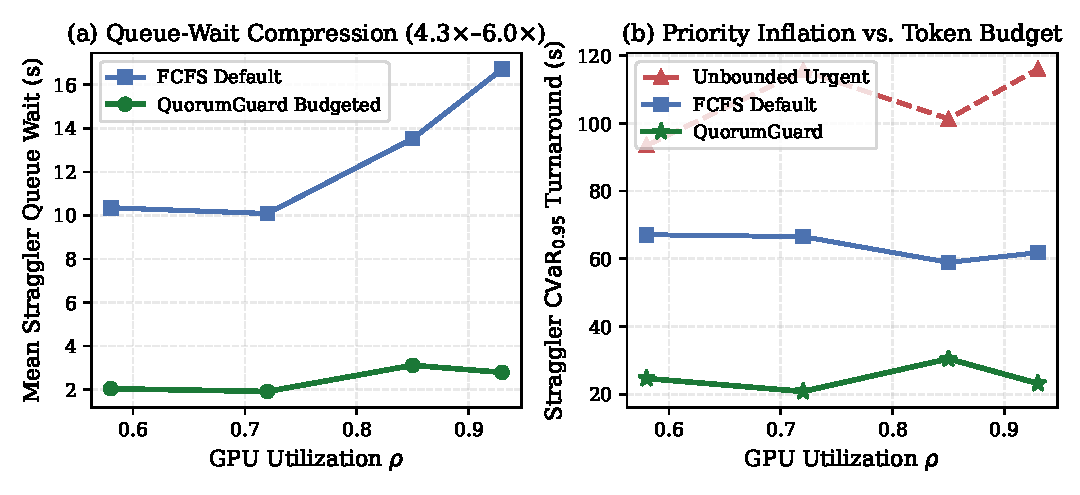
\includegraphics[width=0.98\columnwidth]{fig6_priority_contention.pdf}
  \caption{MPS GPU queue contention across server load $\rho \in [0.58, 0.93]$. (a) \QG{} compresses dissenting straggler queue wait by $4.35\times$--$6.01\times$ over FCFS. (b) Unbounded urgent requests cause priority inflation ($\CVaR_{0.95} = 116.0\text{s}$ and $+98.6\%$ normal-traffic $\mathrm{P95}$ delay at $\rho = 0.93$), whereas \QG{}'s token bucket keeps straggler $\CVaR_{0.95} \le 30.5\text{s}$.}
  \label{fig:contention}
\end{figure}

To test Theorem~\ref{thm:optimality}(2) on measured GPU execution quanta, we profiled 8-token KV-cached decode steps on \texttt{Qwen2.5-7B} ($\mathrm{FP16}$ mean $554.38~\mathrm{ms}$, $\mathrm{P95}$ $694.50~\mathrm{ms}$, prefill $102.17~\mathrm{ms}$) and ran $450$-request Poisson streams across $\rho \in \{0.58, 0.72, 0.85, 0.93\}$ (Table~\ref{tab:contention}, Fig.~\ref{fig:contention}). Under \texttt{FCFS}, dissenting verifiers wait $10.08\text{s}$--$16.72\text{s}$ in queue. Allowing $65\%$ of turns to request urgent priority without a budget (\texttt{Unbounded Urgent}) drives straggler $\CVaR_{0.95}$ to $116.0\text{s}$ and inflates foreground normal $\mathrm{P95}$ by $+98.6\%$ at $\rho = 0.93$. \QG{}'s token bucket compresses dissenting straggler queue waits by $4.35\times$--$6.01\times$ ($16.72\text{s} \to 2.78\text{s}$ at $\rho = 0.93$).

\emph{Trace Examples:} Per-agent calibration logs~\cite{kadavath2022know,guo2017calibration,boland1989majority} illustrate both paths. On routine task \texttt{R01\_sha256\_bytes}, roots $r_0, r_1, r_2$ all choose \texttt{32 bytes} within $1.48\text{s}$ ($\Delta \in [5.8, 9.4]$, $\Htilde \le 0.009$, $\Neff = 2.39$), firing $\mathrm{CleanFast}$ and finishing both stages in $2.34\text{s}$ versus $23.61\text{s}$ under synchronous barriers ($10.1\times$ faster). On \texttt{T02\_float32\_precision\_stall} (\texttt{np.float32(16777216.0) + 1.0}), fast \texttt{3B} agents split across \texttt{16777316.0} and \texttt{Overflow} ($\Htilde = 0.31$); \texttt{Fast k-of-N} commits \texttt{Overflow} at $0.72\text{s}$, whereas \QG{} blocks Line~6, preempts a sandbox verifier to $\mathrm{Priority} = -10$ at $t = 0.92\text{s}$, verifies \texttt{16777216.0} ($\xi_i = 1, \Htilde = 0.000$), and finishes both stages in $8.8\text{s}$ versus $31.8\text{s}$ synchronous.

% ============================================================================
\section{Discussion and Limitations}\label{sec:discussion}
% ============================================================================

\emph{Free-Form Generation:} When agents produce open-ended patches or prose without fixed options, discrete logit probing can be replaced by semantic-cluster entropy~\cite{kuhn2023semantic,farquhar2024nature} over AST or unit-test equivalence classes among early arrivals, while provenance $\Neff$ and sandbox certificates ($\xi_i = 1$) apply unchanged.

\emph{Lineage Metadata and Shared Blind Spots:} Propagating upstream chunk and summary IDs adds $<128~\mathrm{B}$ per RPC, and memoized root resolution in \texttt{ProvenanceDAG} takes $<15~\mu\mathrm{s}$ per arrival event. If every model tier and sandbox script lacks required domain knowledge (as on the remaining $16\%$ of \QBench{} Stage-1 tasks), holding the quorum gate cannot recover a correct answer, though $\Neff$ deduplication still prevents single-source echo cascades.

% ============================================================================
\section{Conclusion}\label{sec:conclusion}
% ============================================================================

Asynchronous $k$-of-$N$ fast quorums fail in multi-agent LLM committees because completion latency and epistemic accuracy covary positively ($\Cov(T_i, 1 - \varepsilon_i) > 0$). Static fast quorums suffer an order-statistic false-consensus phase transition below $\phicrit$ that compounds across multi-stage workflow DAGs. \QG{} combines pre-commitment semantic entropy gating, provenance-DAG effective quorum sizing ($\Neff$), and token-bucket GPU priority dissent preemption. Across $30$-workflow and $50$-workflow two-stage benchmarks on \texttt{Qwen2.5-3B}, \texttt{7B}, and \texttt{14B-Coder} with live Python sandboxes, \QG{} matches synchronous genealogy-weighted accuracy ($+40.0$--$44.0$ percentage points over fast quorums) while reducing $\mathrm{P95}$ and $\CVaR_{0.95}$ tail latency by $3.19\times$--$3.67\times$.

\section*{Code and Data Availability}
Source code, scheduler modules, and the \QBench{} v1.0 dataset~\cite{syed2026quorumbench} are available under Apache~2.0 at \url{https://github.com/batistado/quorumguard}, \url{https://huggingface.co/batistado/QuorumGuard}, \url{https://huggingface.co/datasets/batistado/QuorumBench}, and \url{https://huggingface.co/spaces/batistado/QuorumGuard-Explorer}. The author declares no competing financial interests.

\bibliographystyle{IEEEtran}
\bibliography{references}

\end{document}
